\subsubsection{Heurística constructiva de cluster-first, route-second, clusterizando con algoritmo de Sweeping}

\subsubsubsection{Medición en base a tamaño del grafo}

La cota de complejidad temporal para esta heurística es $\mathcal{O}(n^{2} * log(n))$, con lo cual se espera visualizar un gráfico con una curva creciente.

\begin{figure}[H]
	\centering
	\begin{minipage}[t]{.45\textwidth}
		\centering
		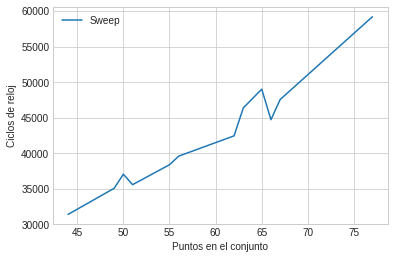
\includegraphics[scale=0.55]{exercise5/sweep3}
	\end{minipage}\qquad
	\begin{minipage}[t]{.45\textwidth}
		\centering
		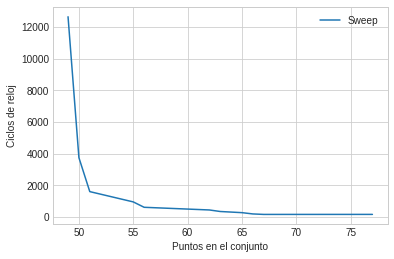
\includegraphics[scale=0.55]{exercise5/sweepAcotado}
	\end{minipage}
\end{figure}

Podemos ver algunas caídas en el gráfico, sin embargo, el contexto general de la curva representa lo esperado. Al dividir los puntos del grafico por la cota, vemos como el grafico converge, significando que la cota propuesta es correcta.


\subsubsubsection{Medición en base a distribución del grafo}

En este caso, se optó por comparar un grafo cuyos puntos estén más agrupados contra otro en el que se encuentren completamente dispersos. Se espera que el caso de los grafos agrupados sea más rápido que el contrario.

\begin{figure}[H]
	\centering
	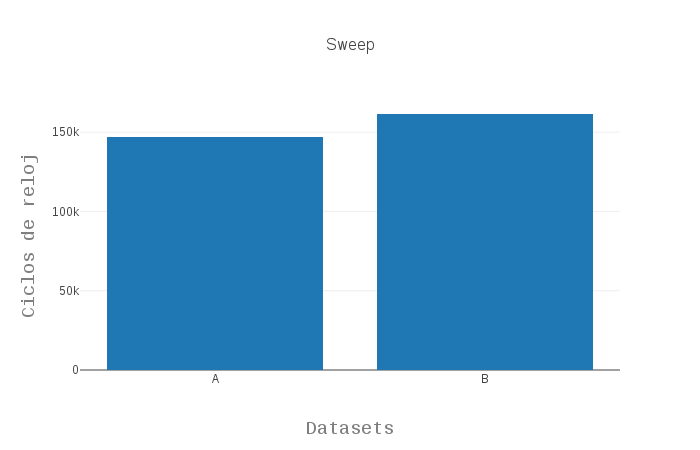
\includegraphics[scale=0.4]{exercise5/sweepType.png}
\end{figure}


No se cumple la suposición.